\documentclass[12pt]{article}

\usepackage{blindtext} % Package to generate dummy text throughout this template 

\usepackage[utf8]{inputenc}
\usepackage{amsmath, amssymb}
\usepackage{algorithm}
\usepackage[noend]{algpseudocode}
\linespread{1.5}
\usepackage[margin = 1in]{geometry}
\usepackage{microtype} % Slightly tweak font spacing for aesthetics
\usepackage[english]{babel} % Language hyphenation and typographical rules
\usepackage{tikz}
\usepackage{pgfplots}
\usepackage{pgfplotstable}
\usepackage{hyperref}
\usepackage{url}
\usepackage{graphicx}
\usepackage{float}
\usepackage{wrapfig}
\usepackage{multicol}
\usepackage{subcaption}
\usepackage{nomencl}
\usepackage[titletoc, page]{appendix}
\usepackage{caption}
\usepackage{setspace}
\captionsetup{font={small, stretch=1}}
\let\Algorithm\algorithm
\renewcommand\algorithm[1][]{\Algorithm[#1]\setstretch{1.5}}
\hypersetup{
    colorlinks=true,
    linkcolor=black,      
    urlcolor=red,
    bookmarks=true,
    citecolor=green!75!black
}

\setlength{\parindent}{2em}
%\setlength{\parskip}{1.5em}
\graphicspath{ {images/} }

% nomenclature specs
\makenomenclature
\renewcommand{\nomname}{List of Commonly Used Functions, Symbols \& Terms}
%% This code creates the groups
% -----------------------------------------
\usepackage{etoolbox}
\renewcommand{\nomgroup}[1]{%
    \item[\bfseries
    \ifstrequal{#1}{T}{Terms}{%
        \ifstrequal{#1}{S}{Symbols}{%
            \ifstrequal{#1}{F}{Functions}{}}%
    }]}
% -----------------------------------------

\newcommand{\vect}[1]{\mathbf{#1}}  % vector
\newcommand{\matr}[1]{\mathbf{#1}}  % matrix
\newcommand{\tens}[1]{\mathbf{#1}}  % tensor
\newcommand{\mean}[1]{\overline{#1}}    % mean overline

\begin{document}
    % nomenclature
    \mbox{}
    % symbols
    \nomenclature[S]{$\matr{M}$; $\matr{m}$}{Matrix or vector depending on the context}
    \nomenclature[S]{$J$}{Number of locations in the dataset}
    \nomenclature[S]{$T$}{Number of time units for which data is available}
    
    % functions
    \nomenclature[F]{softmax($\cdot$)}{Defined as softmax($z_i$) = $\frac{\exp(z_i)}{\sum_{i} \exp(z_i)}$}
    \nomenclature[F]{reLU($\cdot$)}{Defined as reLU($z$) = max(0, $z$)}
    \nomenclature[F]{batch-multiply($\cdot$)}{Operates on $m \times n \times p$ and $m \times p \times q$ tensors to give a $m \times n \times q$ tensor.}
    \printnomenclature[1.5in]
    \cleardoublepage
    
    \tableofcontents
    \listoftables
    \listoffigures
    
    % main body
    \section{Introduction} \label{sec:Introduction}
    Optimizing predictive models on datasets that are obtained from citizen-science projects can be computationally expensive as these datasets grow in size with time. Consequently, models based on multiple-layered neural networks, Integer Programming and other optimization routines can prove increasingly difficult as the number of parameters increase, despite using the faster Central Processing Units (CPUs) in the market. Incidentally, it becomes difficult for citizen-science projects to scale if the organizers use CPUs to run optimization models. However, Graphical Processing Units (GPUs), which offer multiple cores to parallelize computation, can outperform CPUs in computing such predictive models if these models heavily rely on large-scale matrix multiplications. By using GPUs over CPUs to accelerate computation on a citizen-science project, the model could achieve better optimization in less time, enabling the project to scale.
    
    Part of the eBird project, which aims to ``maximize the utility and accessibility of the vast numbers of bird observations made each year by recreational and professional bird watchers'', Avicaching is a incentive-driven game trying to homogenize the spatial distribution of citizens' (agents') observations [cite website]. Since the dataset of agents' observations in eBird is geographically heterogeneous (concentrated in some places like cities and sparse in others), Avicaching homogenizes the observation set by rewarding agents who visit under-sampled locations \cite{Xue2016Avi1}. To accomplish this task of specifying rewards at different locations based on the historical records of observations, Avicaching would learn the change in agents' behavior when a certain sample of rewards were applied to the set of locations, and then distribute a newer set of rewards across the locations based on those learned parameters \cite{Xue2016Avi2}. This requirement naturally translates into a predictive optimization problem, which is implemented using multiple-layered neural networks and linear programming.

    \subsection{Computation Using GPUs} \label{sec:comp_using_GPUs}
    
    \section{Problem Formulation} \label{sec:Problem Formulation}
    Since NVIDIA General Purpose GPUs enable faster computation on matrices, accelerated through CUDA and cuDNN, both the Identification (Section \ref{sec:Identification Problem}) and the Pricing Problem (Section \ref{sec:Pricing Problem}) were formulated as 3-layered and 2-layered neural networks respectively, using the PyTorch library.
    
    \subsection{Identification Problem} \label{sec:Identification Problem}
    As discussed in Section \ref{sec:Introduction}, the model should learn parameters that caused the change in agents' behavior when a certain set of rewards was applied to locations in the experiment region. Specifically, given datasets $\vect{y_t}$ and $\vect{x_t}$ of agents' visit densities with and without the rewards $\vect{r_t}$, we want to find weights $\matr{w_1}$ and $\matr{w_2}$ that caused the change from $\vect{x_t}$ to $\vect{y_t}$, factoring in possible influence from environmental factors $\matr{f}$ and distances between locations $\matr{D}$. Although the original model proposed to learn a single set of weights $\matr{w}$ \cite{Xue2016Avi2}, this proposed model considers two sets of weights $\matr{w_1}$ and $\matr{w_2}$ as it may theoretically result into higher accuracy and lower loss. Mathematically, the model can be formulated as:
    \begin{equation} \label{eq:iden_problem}
    \begin{aligned}
    & \underset{\matr{w_1}, \matr{w_2}}{\text{minimize}}
    & & Z_I(\matr{w_1}, \matr{w_2}) = \sum_{t} (\omega(\vect{y_t} - \matr{P}(\matr{f}, \vect{r_t}; \matr{w_1}, \matr{w_2})\vect{x_t}))^{2}
    \end{aligned}
    \end{equation}
    where $\omega$ is a set of weights at time $t$ capturing penalties relative to the importance of homogenizing at different locations and elements $p_{u, v}$ of $\matr{P}$ are given as:
    \begin{equation} \label{eq:puv_equation}
    p_{u, v} = \frac{\exp(\matr{w_2} \cdot \text{reLU} (\matr{w_1} \cdot [d_{u, v}, \vect{f_{u}}, r_{u}]))}{\sum_{u'} \exp(\matr{w_2} \cdot \text{reLU} (\matr{w_1} \cdot [d_{u', v}, \vect{f_{u'}}, r_{u'}]))} = \frac{\exp(\Gamma_{u, v})}{\sum_{u'}\exp(\Gamma_{u', v})} = \text{softmax}(\Gamma_{u, v})
    \end{equation}
    In the expression for $p_{u,v}$ (Equation \ref{eq:puv_equation}), softmax$(\cdot)$ is the function: softmax$(z_i) = \frac{\exp(z_i)}{\sum_{i}\exp(z_i)}$ and the reLU$(\cdot)$ function is a ``rectified Linear Unit'' defined as: reLU$(z) = \text{max}(0, z)$.
    
    To optimize the loss value $Z_I(\matr{w_1}, \matr{w_2})$ (Equation \ref{eq:iden_problem}), the neural network learns the set of weights through multiple epochs \nomenclature[T]{Epoch}{One training/testing period; iteration}of backpropagating the loss using gradient descent. Furthermore, the program processes the dataset before feeding to the network to avoid unnecessary sub-epochs and promote batch operations on matrices. 
    
    \subsubsection{Structure of Input Dataset for Identifying Weights} \label{sec:Structure of Input Dataset for Identifying Weights}
    \begin{figure}[H]
        \begin{subfigure}{.64\textwidth}
            \centering
            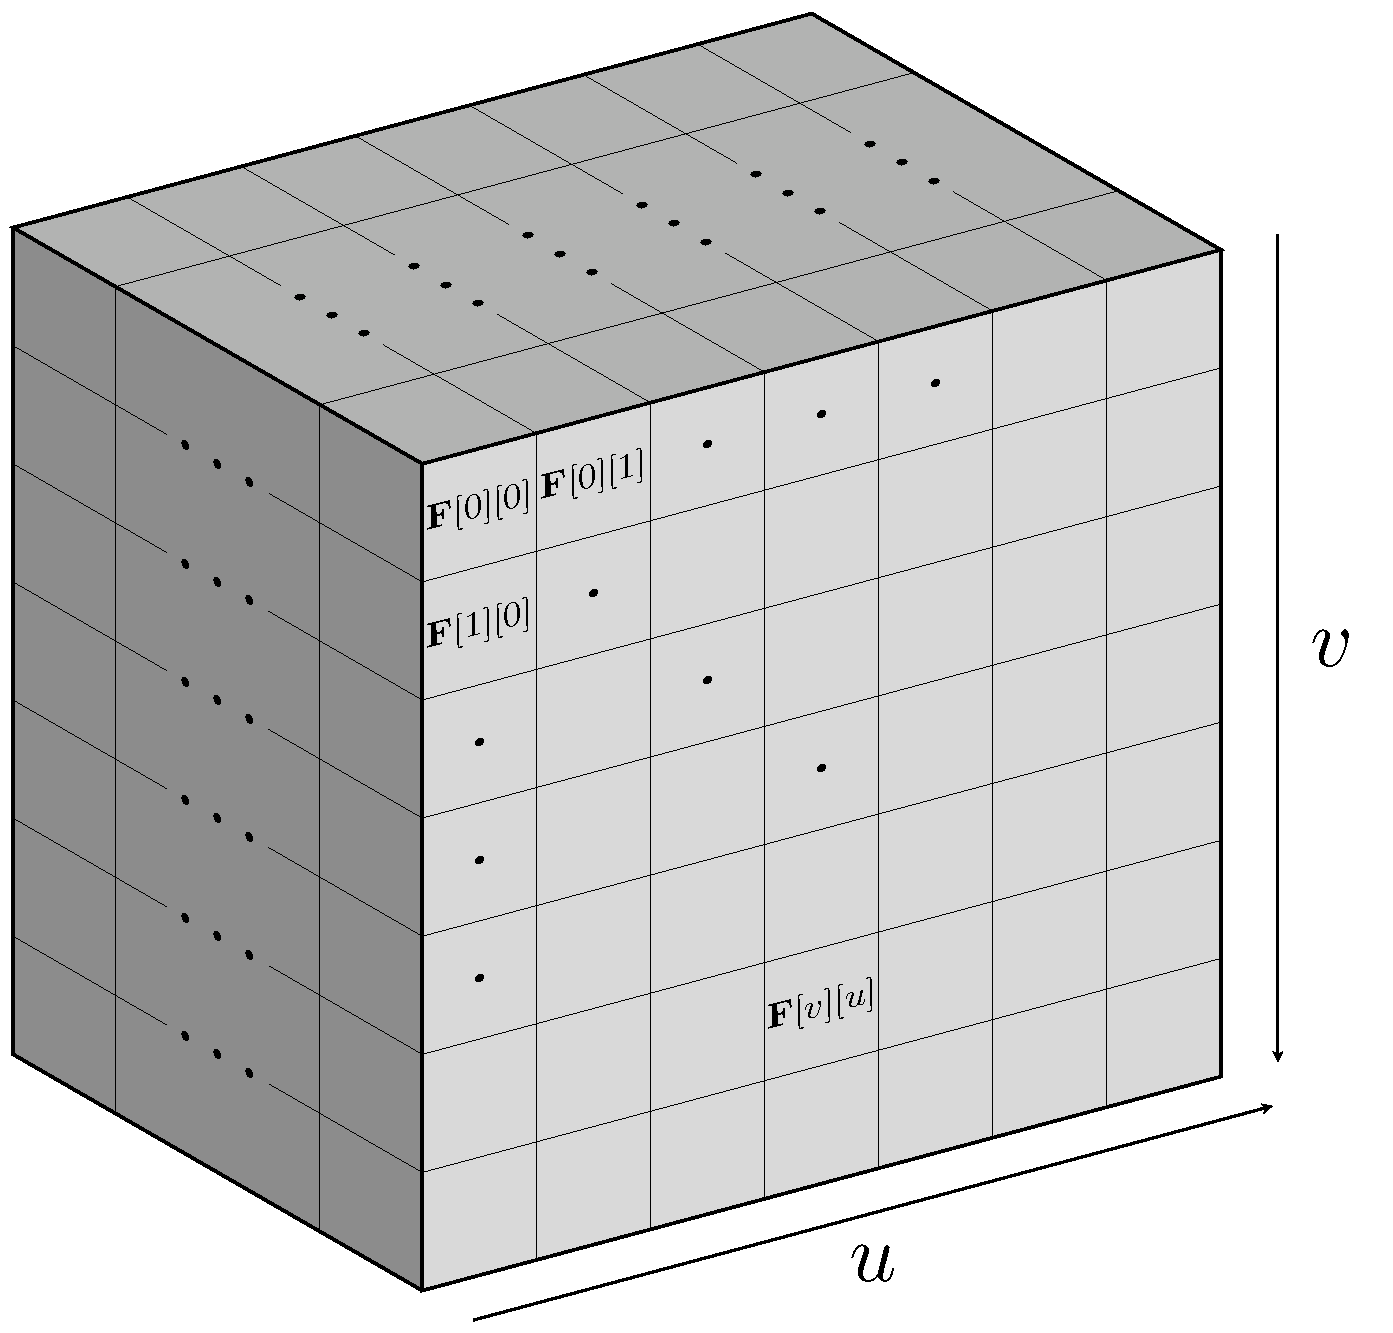
\includegraphics[width=\linewidth]{weights_input_dataset}
            \caption{A Tensor representing the Input Dataset $\matr{F}$}
            \label{fig:A Tensor representing the complete Input Dataset}
        \end{subfigure}
        \begin{subfigure}{.35\textwidth}
            \centering
            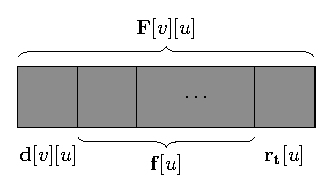
\includegraphics[width=\linewidth]{zoomup_Fuv}
            \caption{Contents of $\matr{F}[v][u]$}
            \label{fig:Zoomed-in contents of Fvu}
        \end{subfigure}
        \caption{Visual representation of the Input Dataset}
        \label{fig:Visual representation of the Input Dataset}
    \end{figure}
    Since preprocessing the dataset impacts the efficiency of the network, the input dataset, comprising of distance between locations $\matr{D}$, environmental features $\vect{f}$ and given rewards $\vect{r_t}$ (all normalized) are combined in a specific manner. Since GPUs are efficient in operating on matrices and tensors, the input dataset is built into a tensor (Figure \ref{fig:A Tensor representing the complete Input Dataset}) such that batch operations could be performed on slices $\matr{F}[v]$. Another advantage of building the dataset as a tensor comes with the PyTorch library, which provides convenient handling and transfer of tensors residing on CPUs and GPUs. Algorithm \ref{alg:Constructing the Input Dataset} describes the steps to construct this dataset.
    \begin{algorithm}
        \caption{Constructing the Input Dataset} \label{alg:Constructing the Input Dataset}
        \begin{algorithmic}[1]
            \Function{Build-Dataset}{$\matr{D}, \matr{f}, \matr{r_t}$}
            \State $\matr{D} \gets \Call{Normalize}{\matr{D}}$\Comment{$\matr{D}[u][v]$ is the distance between locations $u$ and $v$}
            \State $\vect{f} \gets \Call{Normalize}{\mathbf{f}, axis = 0}$\Comment{$\mathbf{f}[u]$ is a vector of env. features at location $u$}
            \State $\vect{r_t} \gets \Call{Normalize}{\vect{r_t}, axis = 0}$\Comment{$\vect{r_t}[u]$ is the reward at location $u$}
            \For{$v = 1, 2, \dots, J$}
                \For{$u = 1, 2, \dots, J$}
                    \State $\tens{F}[v][u] \gets [\matr{D}[v][u], \vect{f}[u], \vect{r_t}[u]]$ \Comment{As depicted in Figure \ref{fig:Zoomed-in contents of Fvu}}
                 \EndFor
            \EndFor
            \State \Return $\matr{F}$
            \EndFunction
        \end{algorithmic}
    \end{algorithm}
       
    \subsubsection{Minimizing Loss for the Identification Problem} \label{sec:Minimizing Loss for the Identification Problem}
    As shown in Figure \ref{fig:Neural network designed for the Identification Problem}, the neural network is made of 3 fully connected layers - the input layer, the hidden layer with rectified Linear Units (reLU), and the output layer generating the results using the softmax$(\cdot)$ function. The network can also be visualized as a collection of 1-dimensional layers (Figure \ref{fig:Side view of the network}), with the softmax$(\cdot)$ calculated on the collection's output.
    \begin{figure}[H]
        \begin{subfigure}{.64\textwidth}
        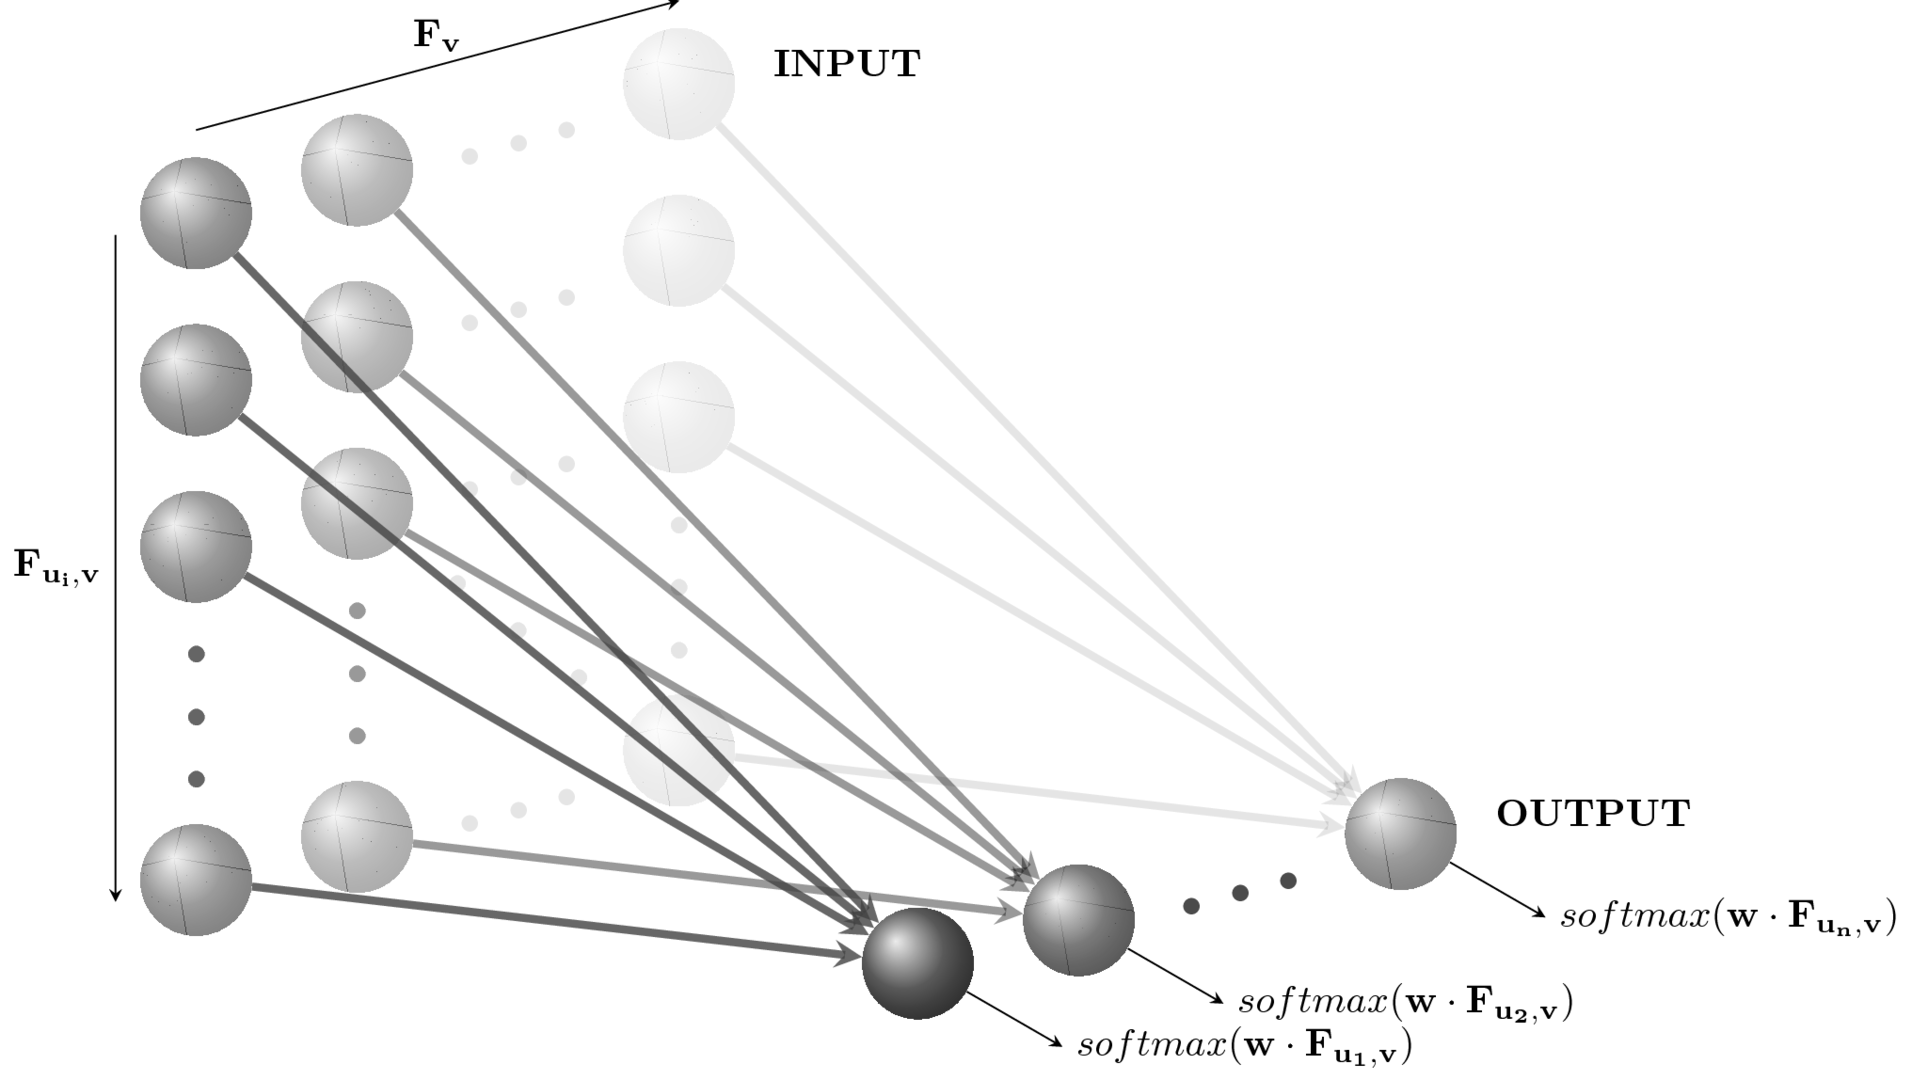
\includegraphics[width=\textwidth]{weights_net}
        \caption{3-dimensional view of the network slice, taking in $\matr{F}[v]$}
        \label{fig:3-dimensional view of the network slice, taking in Fv}
        \end{subfigure}
        \begin{subfigure}{.35\textwidth}
            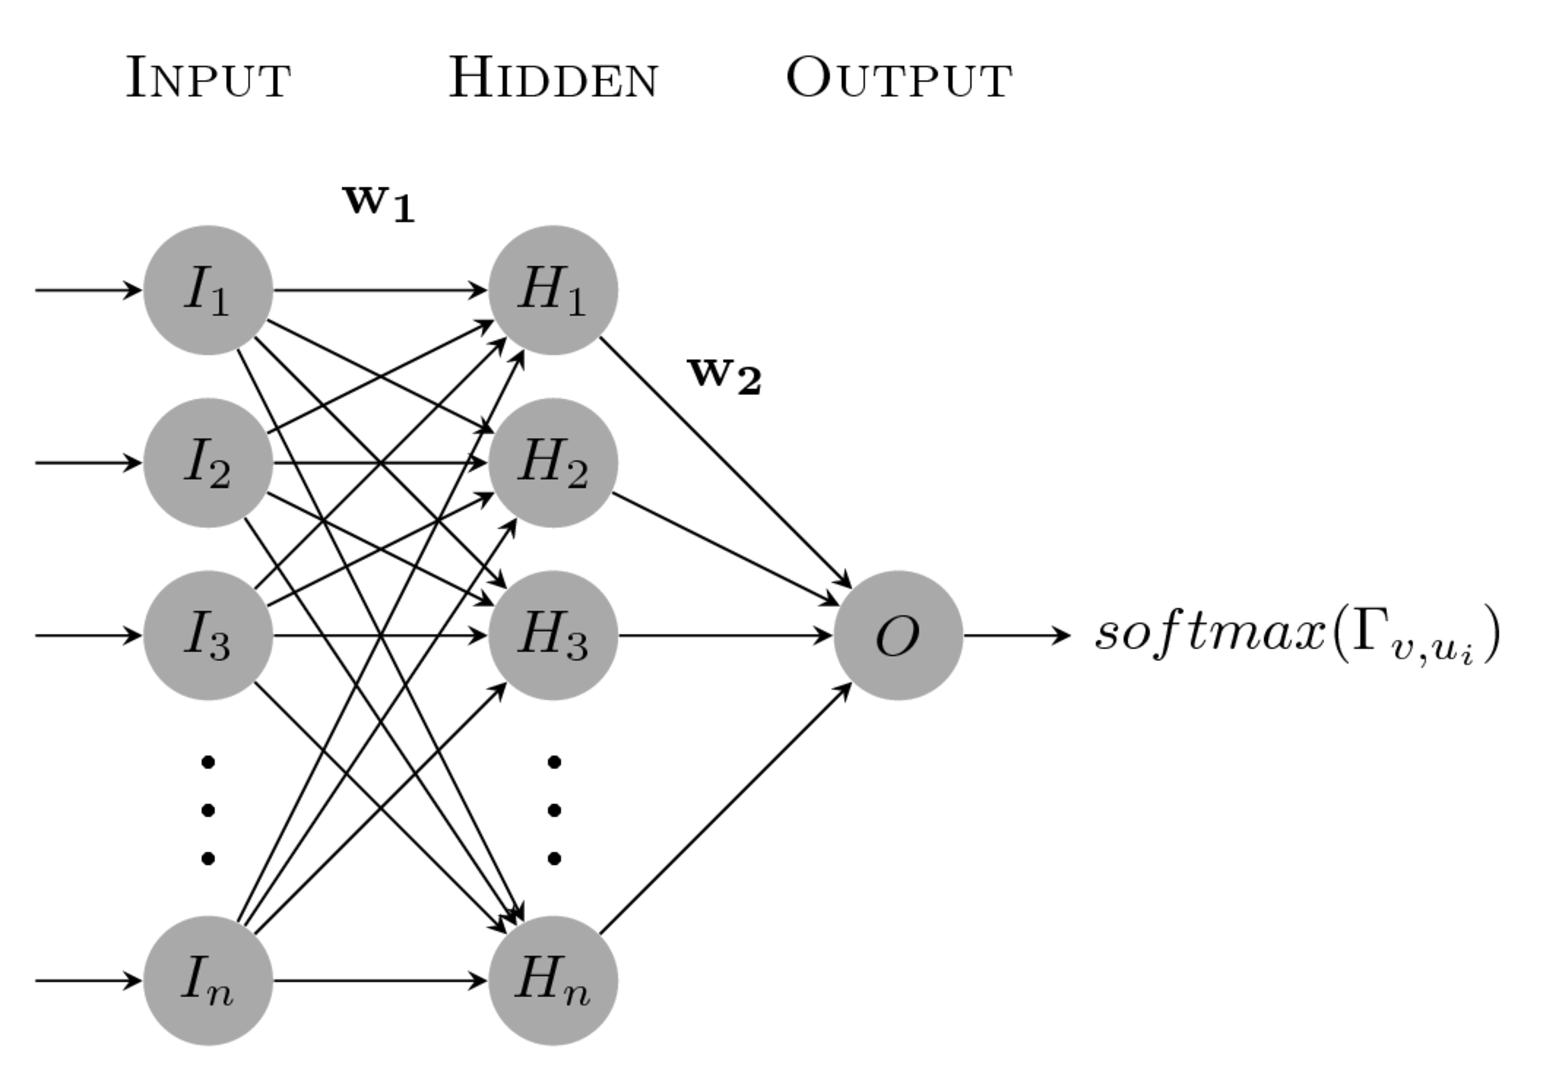
\includegraphics[width=\textwidth]{weights_net_side}
            \caption{Side view of the network}
            \label{fig:Side view of the network}
        \end{subfigure}
        \caption{Neural network designed for the Identification Problem}
        \label{fig:Neural network designed for the Identification Problem}
    \end{figure}
    It is important to clarify that the network in Figure \ref{fig:3-dimensional view of the network slice, taking in Fv}, which takes in $\matr{F}[v]$ as shown, is a slice of the original network, which takes in the complete tensor $\matr{F}$ and computes the complete result $\matr{P}^{T}$  per iteration of $t$. In other words, the input and the hidden layers are 3-dimensional, and the output layer is 2-dimensional. Since it is difficult to visualize the complete network on paper, slices of the network are depicted in Figure \ref{fig:3-dimensional view of the network slice, taking in Fv}. Algorithm \ref{alg:Algorithm for the Identification Problem per epoch} details the steps for learning the parameters $\matr{w_1}$ and $\matr{w_2}$ based on Equations \ref{eq:iden_problem} \& \ref{eq:puv_equation}.
    \begin{algorithm}
        \caption{Algorithm for the Identification Problem per epoch} \label{alg:Algorithm for the Identification Problem per epoch}
        \begin{algorithmic}[1]
            \Require $\matr{w_1}, \matr{w_2}, T$
            \Function{Identify-Weights}{$\matr{x}, \matr{y}, \matr{r}, \matr{D}, \matr{f}, \omega$}
            \For{$t = 1, 2, \dots, T$}
                \State $\matr{F} \gets \Call{Build-Dataset}{\matr{D}, \matr{f}, \matr{r}[t]}$\Comment{Defined in Algorithm \ref{alg:Constructing the Input Dataset}}
                \State $\matr{\Lambda} \gets \text{reLU}(\Call{Batch-Multiply}{\matr{F}, \matr{w_1}})$\Comment{\textbf{Phase 1: Feed Forward}}
                \State $\matr{\Gamma} \gets \text{softmax}(\Call{Batch-Multiply}{\matr{\Lambda}, \matr{w_2}})$
                \State $\matr{P} \gets \matr{\Gamma}^T$
                \State $loss \gets loss + (\omega(\matr{y}[t] - \matr{P} \cdot \matr{x}[t]))^2$
            \EndFor
            \State $\Call{Gradient-Descent}{loss, \matr{w_1}, \matr{w_2}}$\Comment{\textbf{Phase 2: Backpropagate}}
            \State $\matr{w_1}, \matr{w_2} \gets \Call{Update-Using-Gradients}{\matr{w_1}, \matr{w_2}}$
            \State \Return $loss$
            \EndFunction
        \end{algorithmic}
    \end{algorithm}
    
    \subsection{Pricing Problem} \label{sec:Pricing Problem}
    After learning the set of weights $\matr{w_1}$ and $\matr{w_2}$ highlighting the change in agents' behavior to collect observations, the Pricing Problem aims to redistribute rewards to the all locations such that the predicted behavior of agents influenced by the new set of rewards is homogeneous. Thus, given a budget of rewards $\mathcal{R}$, this optimization problem can be expressed as:
    \begin{equation} \label{eq:pricing_problem}
    \begin{aligned}
    & \underset{\vect{r}}{\text{minimize}}
    & & Z_P(\vect{r}) = \frac{1}{n}\lVert \vect{y} - \mean{\vect{y}} \rVert\\
    & \text{subject to}
    & & \vect{y} = \matr{P}(\matr{f}, \vect{r}; \matr{w_1}, \matr{w_2}) \, \vect{x}\\
    &&& \sum_{i} r_i \leq \mathcal{R}\\
    &&& r_i \geq 0
    \end{aligned}
    \end{equation}
    where elements of $\matr{P}$ are defined as in Equation \ref{eq:puv_equation}.
    
    To allocate the rewards $\vect{r}$ optimally, the calculations for the pricing problem are akin to that for the Identification Problem (Section \ref{sec:Identification Problem}). However, since only 1 set of rewards need to be optimized, we use an altered 2-layer network instead of the 3-layer network used to identify the weights. While Equation \ref{eq:pricing_problem} looks like a typical Linear Programming problem, only a part of the formulation uses Linear Programming to constrain the rewards. The more computationally expensive part (calculation for $\matr{P}$ on a CPU) is modeled as a 2-layer network that minimizes the loss function $Z_P(\vect{r})$ using gradient descent. Although this use of a neural network may seem similar to that of the Identification Problem, there are major changes in the structure of the network used here. These alterations for the Pricing Problem and differences from the Identification Problem are discussed further in the following sections.
    
    \subsubsection{Input Dataset for Finding Rewards}
    
    Since it is the set of rewards $\vect{r}$ that need to be optimized, they must serve as the ``weights'' of the network (note that ``weights'' refer to the edges of this network and not to the set of calculated weights $\matr{w_1}$ and $\matr{w_2}$). Therefore, the rewards $\vect{r}$ are no longer fed into the network but are its characteristic. Instead, the calculated weights $\matr{w_1}$ are fed into the network, and are ``weighted'' by the rewards.
    
    The observation density datasets, $\matr{x}$ and $\matr{y}$, are also aggregated for all agents such that they give information in terms of locations $u$ only. This is also why rewards $\vect{r}$ does not depend on $t$ - we want a generalized set of rewards for all time $t$ per location $u$. Therefore, the algorithm for constructing $\matr{F}$ (Section \ref{sec:Structure of Input Dataset for Identifying Weights}) is same as Algorithm \ref{alg:Constructing the Input Dataset} but with a change - $\vect{r_t}$ replaced by $\vect{r}$.
    
    \subsubsection{Optimizing \& Constraining Rewards} \label{sec:Optimizing and Constraining Rewards}
    The algorithm for finding $\matr{P}$ is very similar to Phase 1 of Algorithm \ref{alg:Algorithm for the Identification Problem per epoch} but without any epochs of $t$, as $\vect{x}$ is a vector rather than a matrix. Also, since the program would predict $\vect{y}$, it does not need labels $\vect{y}$ as a dataset.
    
    \begin{algorithm}
        \caption{Solving the Pricing Problem} \label{alg:Solving the Pricing Problem}
        \begin{algorithmic}[1]
            \Function{Optimize-Rewards}{$\vect{x}, \matr{w_1}, \matr{w_2}, \matr{D}, \matr{f}$}
            \Require $\vect{r}, \mathcal{R}$
            \State $\matr{F} \gets \Call{Build-Dataset}{\matr{D}, \matr{f}, \vect{r}}$\Comment{Defined in Algorithm \ref{alg:Constructing the Input Dataset}}
            \State $\matr{\Lambda} \gets \text{reLU}(\Call{Batch-Multiply}{\matr{F}, \matr{w_1}})$\Comment{\textbf{Phase 1: Solve for $\matr{P}$ and $loss$}}
            \State $\matr{\Gamma} \gets \text{softmax}(\Call{Batch-Multiply}{\matr{\Lambda}, \matr{w_2}})$
            \State $\matr{P} \gets \matr{\Gamma}^T$
            \State $\vect{y} \gets \matr{P} \cdot \vect{x}$
            \State $loss \gets \lVert \vect{y} - \mean{\vect{y}} \rVert / J$\Comment{$J$ is the number of locations}
            \State $\Call{Gradient-Descent}{loss, \vect{r}}$\Comment{\textbf{Phase 2: Backpropagate}}
            \State $\vect{r} \gets \Call{Update-Using-Gradients}{\vect{r}}$
            \State $\vect{r} \gets \Call{LP}{\vect{r}, \mathcal{R}}$\Comment{LP($\cdot$) explained below}
            \State \Return $loss$
            \EndFunction
        \end{algorithmic}
    \end{algorithm}
    After updating the rewards, the program constrains them using LP($\cdot$) such that $\sum_{i}r_i \leq \mathcal{R}$ and $r_i \geq 0$. To do so, the LP($\cdot$) finds another set of rewards $\vect{r'}$ such that the absolute difference between new and old rewards ($\sum_{i}|r'_i - r_i|$) is minimum. The mathematical formulation is given in Equation \ref{eq:lp_math_constrain_rewards}, which was implemented using SciPy's Optimize Module []. Since the module supports a standard format\footnote{minimize [$\vect{c}^T \cdot \vect{x}$]; subject to [$\matr{A} \cdot \vect{x} \leq \vect{b}, \, x_i \geq 0$] \label{foot:lp standard format}} for doing linear programming, Equation \ref{eq:lp_code_constrain_rewards} (after rearranging constraints and building $\matr{A}, \vect{b}$ and $\vect{c}$) is used, which is mathematically equivalent to Equation \ref{eq:lp_math_constrain_rewards}.
    \begin{multicols}{2}
        \begin{equation} \label{eq:lp_math_constrain_rewards}
        \begin{aligned}
            & \underset{\vect{r'}}{\text{minimize}}
            & & \sum_{i}|r'_i - r_i|\\ \\
            & \text{subject to}
            & & \sum_{i}r'_i \leq \mathcal{R}\\
            &&& r_i \geq 0
        \end{aligned}
        \end{equation}\break
        \begin{equation} \label{eq:lp_code_constrain_rewards}
        \begin{aligned}
            & \underset{\vect{r'}, \vect{u}}{\text{minimize}}
            & & \sum_{i} u_i\\
            & \text{subject to}
            & & r'_i - r_i \leq u_i\\
            &&& r_i - r'_i \leq u_i\\
            &&& \sum_{i} r'_i \leq \mathcal{R}\\
            &&& r'_i, u_i \geq 0
        \end{aligned}
        \end{equation}
    \end{multicols}

    \section{Experiment Specifications} \label{sec:Experiment Specifications}
    To test both our models, we conducted several tests for optimization and GPU speedup over CPU. After initializing all parameters randomly and reading data from files, the models were run for 1000 to 10000 epochs depending on the complexity of the model and any potential benefits emerging with more epochs.
    
    A Dell Precision Tower 3620 with Intel Core i7-7700K Processor, 16GB RAM and NVIDIA Quadro P4000 GPU with 1792 CUDA Cores was used for all experiments, which were run on original datasets for optimization tests and randomly generated datasets for GPU speedup tests. We believe that speedup tests on original datasets would give similar results, though we used randomly generated datasets because it was easier to scale the sizes of random data and test on a variety of dataset sizes.
    
    Note that operations in the scripts were distributed between CPU and GPU when GPU is mentioned as ``set'', while the operations were executed only on the CPU when the ``CPU'' is mentioned as set. Since GPUs are inferior than CPUs at handling most operations other than simple arithmetic matrix ones, we used - and recommend using - both the CPU and the GPU in the former case (GPU ``set'') to handle operations they are superior at. However, since the models in Sections \ref{sec:Identification Problem} and \ref{sec:Pricing Problem} (not the full scripts) are primarily arithmetic operations on matrices and tensors, it is clear that they were executed on the GPU when it was ``set'' and on the CPU when the CPU was ``set''.
    
    On the algorithm side, we used Adam's algorithm for \textsc{Gradient-Descent}($\cdot$), after testing performances of several algorithms including but not limited to Stochastic Gradient Descent (SGD) [], Adam's Algorithm [] and RMSProp [] (PyTorch lets you choose the corresponding function). Since Adam's algorithm was found to work best with both models over all test runs, all experiments were done using Adam's algorithm.
    
    \subsection{Running the Identification Problem's Model}
    \subsubsection{Optimizing the Original Dataset}
    The 3-layered neural network was run for 10000 epochs on the original dataset, which was split 80:20 for training and testing sets, with learning rate = 0.01. Since we were aiming for optimization, we ran multiple tests (5 different seeds) of the model only with the GPU ``set''.
    
    To compare this model's optimization results with other model structures, the previously studied 2-layered network \cite{Xue2016Avi2} and a 4-layered neural network were used. The 4-layered network had another hidden layer with reLU, equivalent to the hidden layer in the current 3-layered network (Figure \ref{fig:3-dimensional view of the network slice, taking in Fv}). The results from the 2-layered network were obtained from the study, and those from the 4-layered network were attained on the same original dataset with same parameter values (learning rate, epochs etc.).
    
    \subsubsection{Testing GPU Speedup on the Random Dataset}
    After generating random datasets of different sizes ($T = 17, 85, 173$ - Section \ref{sec:Minimizing Loss for the Identification Problem}, we ran our 3-layered model on each dataset size with different seeds with both GPU and CPU ``set''.
    
    \subsection{Running the Pricing Problem's Model}
    \subsubsection{Optimizing the Original Dataset}
    After obtaining the set of weights $\matr{w_1}$ and $\matr{w_2}$ optimized using different seeds, we tested to find the best rewards (with the lowest loss - Equation \ref{eq:pricing_problem}) with random $\vect{r}$ initiation. To average the results, the model was run several times on the same set of weights, using different set of weights (obtained from running the Identification Problem with different seeds) each time. Specifically, we ran the Pricing Problem's model 5 times (each with different seeds) for each set of weights, which were itself 5 in number.
    
    Two sets of rewards were tested for loss values as baseline comparisons to our model - a randomly generated set, and another with elements proportionate to the reciprocal of number of visits at each location. While the former was a random baseline, the latter captured the idea of allocating higher rewards to relatively under-sampled locations. The average loss values were compared for all tests with the baselines.
    
    \subsubsection{Testing GPU Speedup on the Random Dataset}
    After generating random datasets of different sizes ($J = 11, 55, 116$ - Section \ref{sec:Minimizing Loss for the Identification Problem}), we ran our 3-layered model on each dataset size with different seeds with both GPU and CPU ``set''.
    
    Since PyTorch does not provide a GPU-accelerated Simplex LP solver, we relied on SciPy's Optimize Module to solve the that part of the model. Since SciPy's implementation does not utilize the GPU \textit{conspicuously}, we expected the Linear Programming part to be executed on the CPU and thus deliver equivalent results in both GPU and CPU ``set'' configurations.
    
    \section{Results} \label{sec:Results}
    \subsection{Identification Problem's Results}
    Minimizing the loss function in the Identification Problem (Section \ref{sec:Identification Problem}) on the original dataset for 10000 epochs took an average of 1260.62 seconds with the GPU ``set''.
    \begin{itemize}
        \item The average loss values at the end of 10000 epochs were 0.04 on the training set and 0.14 on the test set.
        \item The average loss values for the 4-layered model (for comparison) with same experiment specifications were 0.14 on the training set and 0.49 on the test set.
    \end{itemize}
    \begin{wrapfigure}{r}{.5\textwidth}
        \centering
        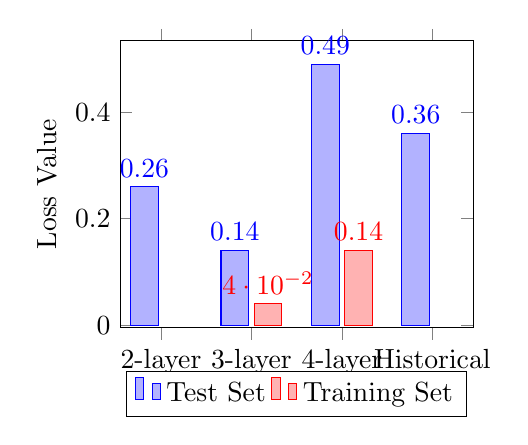
\begin{tikzpicture}
        \begin{axis}[
        ybar,
        width=.5\textwidth,
        enlarge x limits=0.15,
        legend style={at={(0.5,-0.15)},
            anchor=north,legend columns=-1},
        ylabel={Loss Value},
        symbolic x coords={2-layer,3-layer,4-layer, Historical},
        xtick=data,
        nodes near coords,
        nodes near coords align={vertical},
        ]
        \addplot coordinates {(2-layer,0.26) (3-layer,0.14) (4-layer,0.49) (Historical, 0.36)};
        \addplot coordinates {(3-layer,0.04) (4-layer,0.14)};
        \legend{Test Set,Training Set}
        \end{axis}
        \end{tikzpicture}
        \caption[Comparison of Loss Values from Different Models of the Identification Problem]{Comparison of Loss Values from Different Models of the Identification Problem: Loss values for the training set are inevitably lower than that for the test set, which should be the basis for comparison}
        \label{fig:Comparison of Loss Values from Different Models of the Identification Problem}
    \end{wrapfigure}

    As depicted in Figure \ref{fig:Comparison of Loss Values from Different Models of the Identification Problem}, our 3-layered neural network outperformed the previous 2-layered model by 0.12 units (12\% more closer to Ground Truth \cite[Table 1]{Xue2016Avi2}), and also produced much better results (35\% more closer to Ground Truth) than the 4-layered model.
    
    Although there remained a 10\% difference (0.10 loss units) in the values of training and testing set, the 3-layered model was not starkly overfitting as an average \textit{end} difference of $10.7\pm5.5\%$ persisted for many epochs, instead of increasing and tuning more to the training set. On the other hand, overfitting is more remarked in the case of 4-layered model, producing an average \textit{end} difference of $34.8\pm8.9\%$, but erratically hovering between 20\% and 50\%. This result is shown in Figure \ref{fig:Train & Test Loss Values' Plots of Different Models} with plots of loss values at each epoch for the 3- and the 4-layered network.
    \begin{figure}[h]
        \centering
        \begin{subfigure}{.49\textwidth}
            \centering
            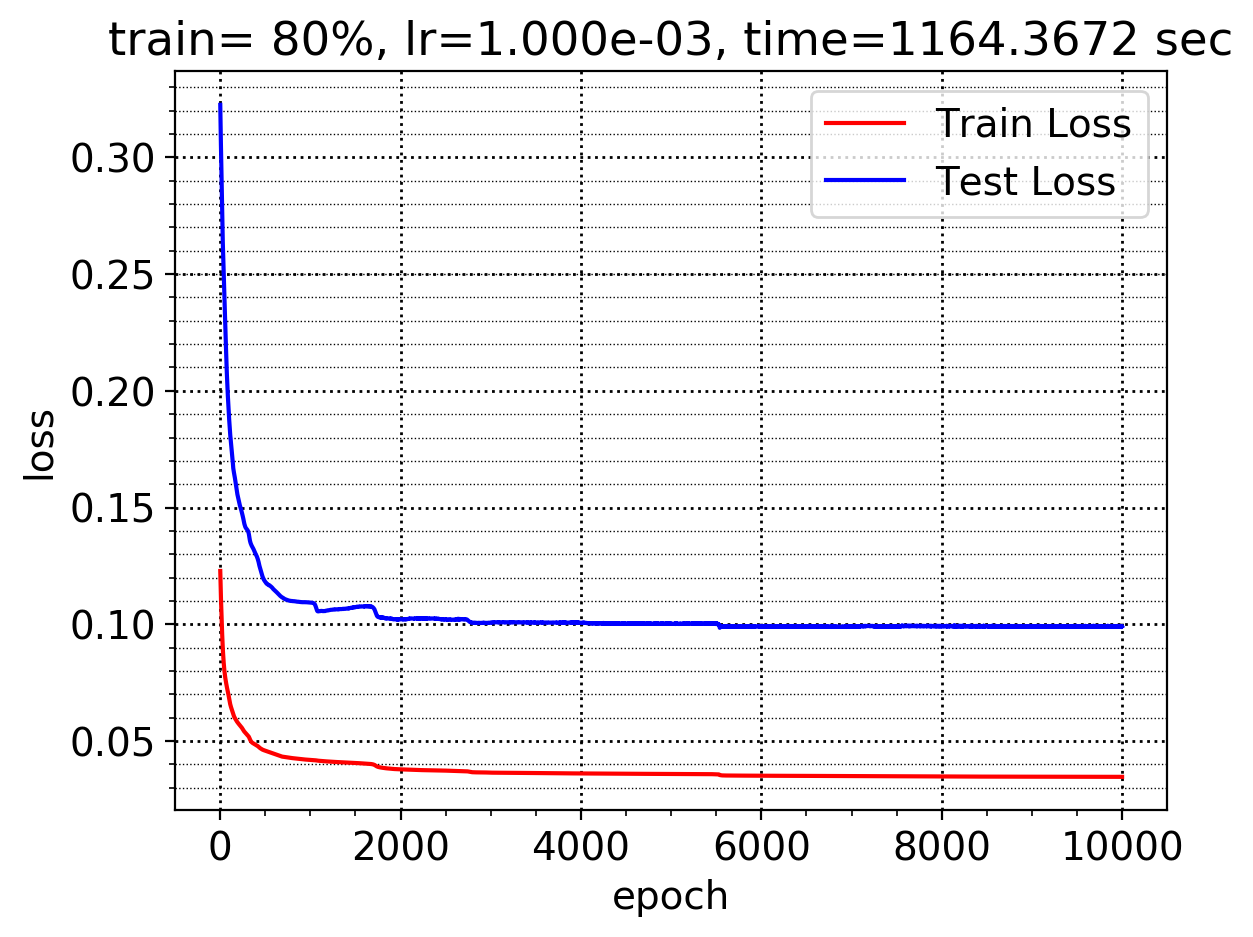
\includegraphics[width=\textwidth]{weights_train_test_loss_3_plot}
            \caption{Plot for 3-layered Model}
            \label{fig:Plot for 3-layered Model}
        \end{subfigure}
        \begin{subfigure}{.49\textwidth}
            \centering
            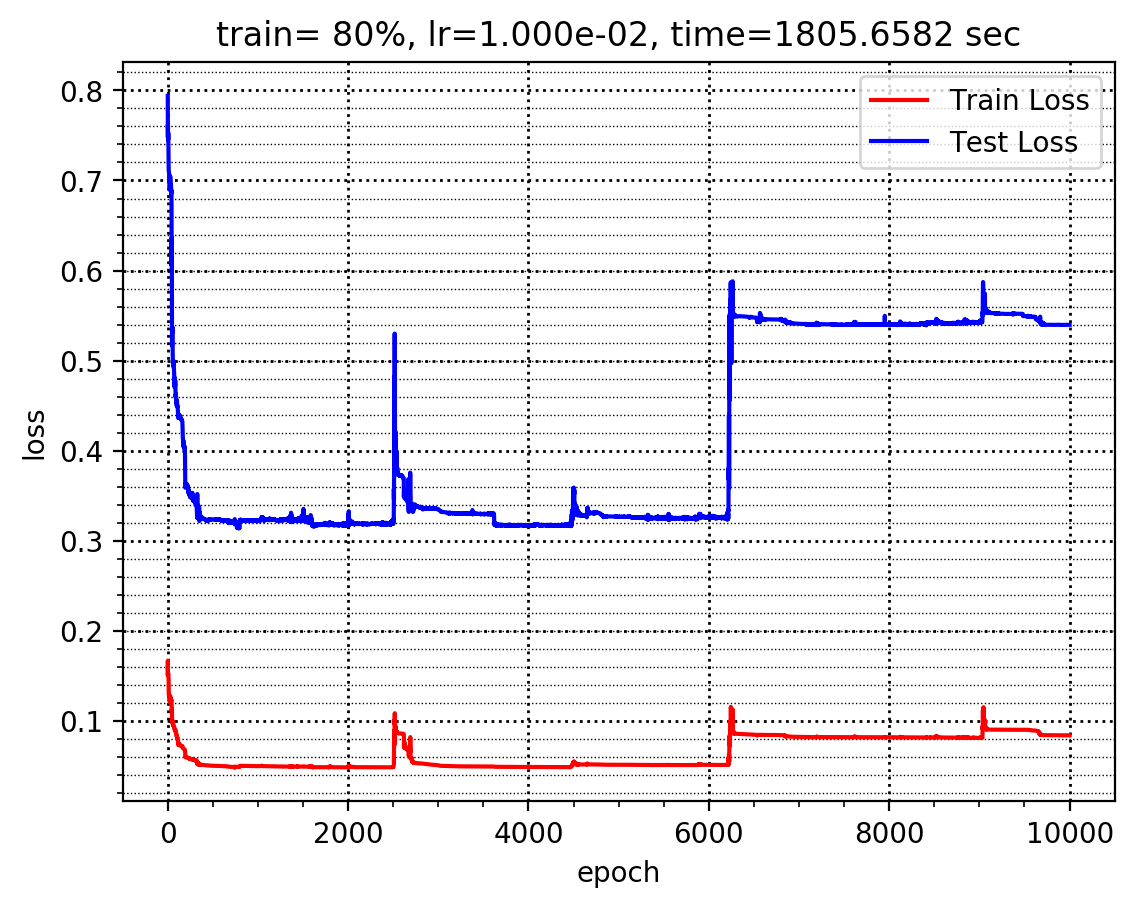
\includegraphics[width=\textwidth]{weights_train_test_loss_4_plot}
            \caption{Plot for 4-layered Model}
            \label{fig:Plot for 4-layered Model}
        \end{subfigure}
        \caption{Train \& Test Loss Values' Plots for One of the Runs of Different Models}
        \label{fig:Train & Test Loss Values' Plots of Different Models}
    \end{figure}

    \begin{wrapfigure}{r}{.4\textwidth}
        \centering
        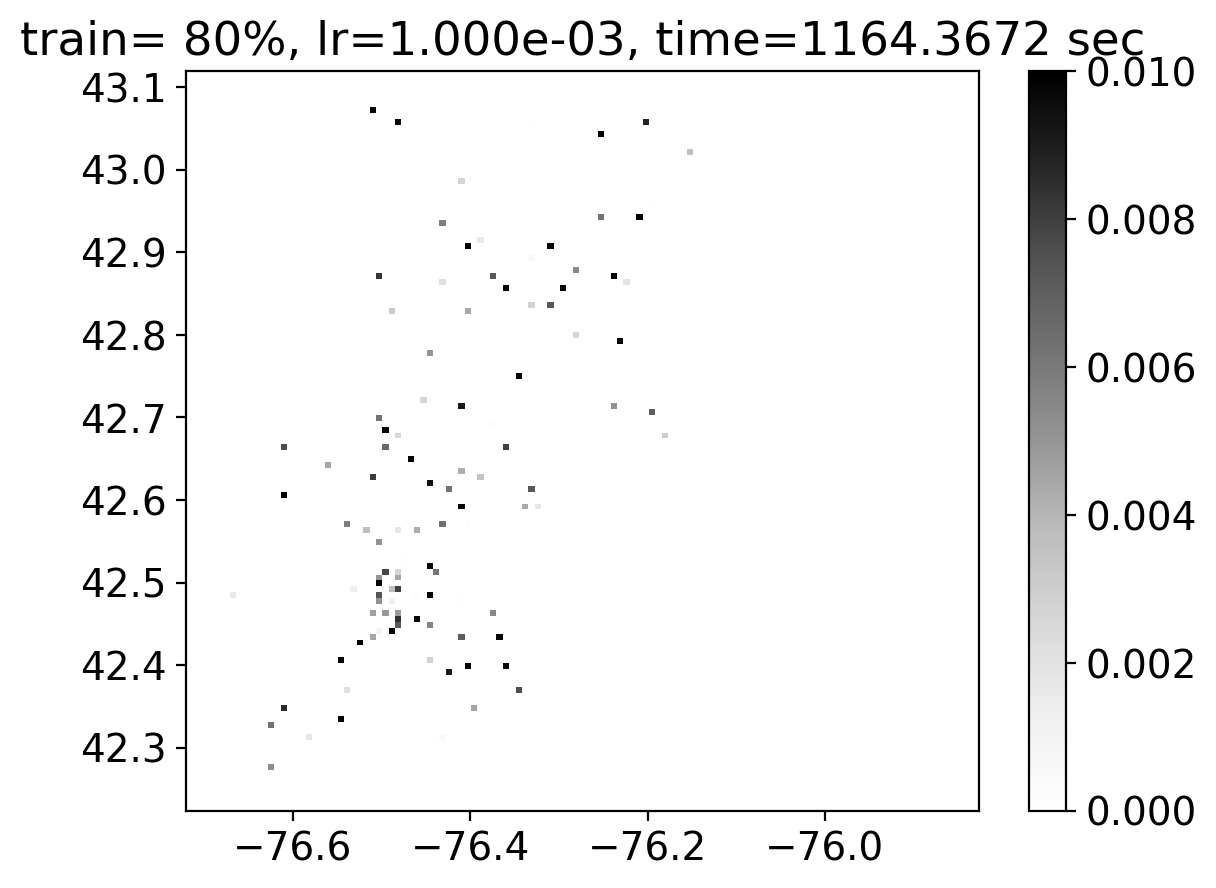
\includegraphics[width=.4\textwidth]{weights_map_plot_3}
        \caption[Predicted Probabilities of Agents Visiting Each Location Plotted on a Map]{Predicted Probabilities of Agents Visiting Each Location Plotted on a Map: Dark dots represent high prediction of visits. Compared to the map plots for the 2-layered network \cite[Figure 3]{Xue2016Avi2}, this plot finds the homogeneity very well.}
        \label{fig:Predicted Probabilities of Agents Visiting Each Location Plotted on a Map}
    \end{wrapfigure} 
    We also generated the predicted probabilities of the agents visiting each location ($\matr{P} \cdot \matr{x}$) in the Test Set, and plotted it onto a map marked by the locations' latitudes and longitudes. Figure \ref{fig:Predicted Probabilities of Agents Visiting Each Location Plotted on a Map} shows such a plot generated by the 3-layered network, where each dot represents a location.
    
    Running on batches of sizes $T = 17, 85, 173$ on a randomly generated dataset, with both GPU and CPU ``set'' separately, we obtained full  execution time (including both training and testing) information. The average results (3 different seeds for each batch) are plotted in Figure \ref{fig:Execution Times of Different Batch-Sizes with GPU and CPU ``set'' Separately}, which show promising GPU speedup over CPU figures for any batch size - for every unit increase in batch-size $T$, CPU ``set'' takes $\approx$ 4.66 seconds, while GPU ``set'' takes only $\approx$ 0.74 more seconds (slopes of best-fit trendlines).
    \begin{figure}[h]
        \centering
        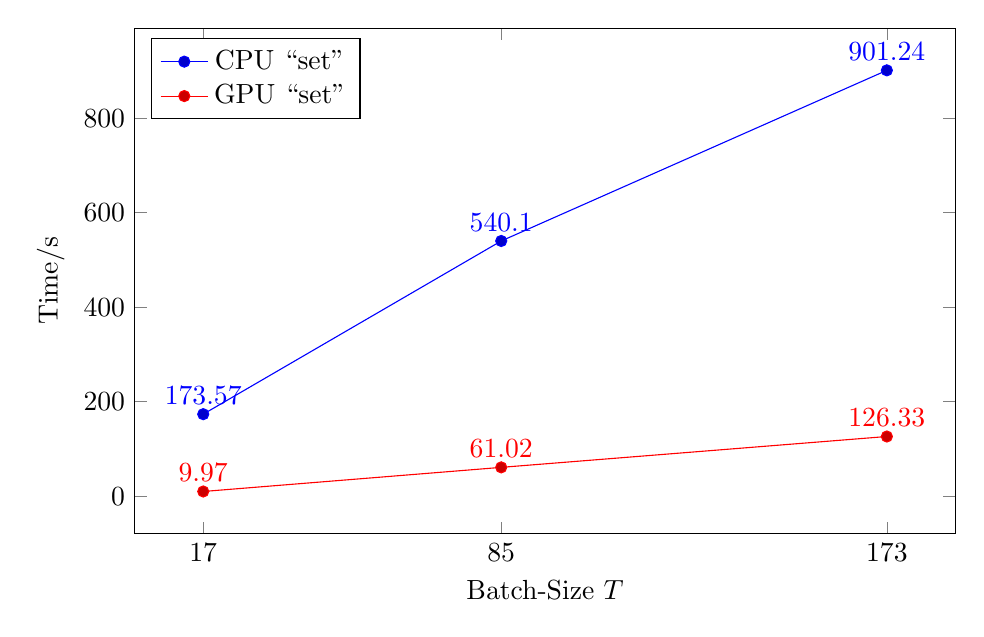
\begin{tikzpicture}
            \begin{axis}[
            width=12cm,
            height=8cm,
            xtick=data,
            xlabel={Batch-Size $T$},
            ylabel={Time/s},
            y tick label style={/pgf/number format/1000 sep=},
            extra y tick style={grid=major, tick label style={xshift=-1cm}},
            legend style={at={(0.02,.98)},
                anchor=north west},
            nodes near coords,
            ]
            \addplot+ [mark=*,] coordinates {(17,173.57) (85,540.10) (173,901.24)};  % cpu
            \addplot+ [mark=*,] coordinates {(17,9.97) (85,61.02) (173,126.33)};  % gpu
            \legend{CPU ``set'',GPU ``set''}
            \end{axis}
        \end{tikzpicture}
        \caption[Execution Times of Different Batch-Sizes with GPU and CPU ``set'' Separately]{Execution Times of Different Batch-Sizes with GPU and CPU ``set'' Separately: Scaling on a GPU is more efficient (about $\frac{4.66}{0.74} \approx 6.25$ times) than doing so on a CPU.}
        \label{fig:Execution Times of Different Batch-Sizes with GPU and CPU ``set'' Separately}
    \end{figure}

    \subsection{Pricing Problem's Results}
    After doing tests on the origina for loss minimization and comparing with the baseline scores, we found that our model was performing $\approx$10 times better than both randomly generated and proportionally distributed rewards. Table [] lists the average loss values obtained on each type of reward allocation (model's predicted, random and proportionate).
    
    After running on different batch-sizes $J = 11, 55, 116$ (the Pricing Problem's model does not iterate over $T$ - Algorithm \ref{alg:Solving the Pricing Problem}), we did not observe profound speedup for the full model. Figure [] shows the decreasing speedup trend, as the GPU ``set'' configuration struggled to complete all epochs faster than with CPU ``set''. The GPU ``set'' config. took $\approx$ 1.42 seconds more for unit increase in batch-size $J$, whereas the CPU ``set'' config. took $\approx$ 2.44 seconds more - a speedup of just 1.72 times.
    
    However, after realizing that the Linear Programming part (Equations \ref{eq:lp_math_constrain_rewards} \& \ref{eq:lp_code_constrain_rewards}) might be influencing these logged times, we recorded running times for both the neural network and the LP separately. As we suspected, the LP did impact the runtimes more than the neural networks did, and the GPU speedup for the neural network was expectedly high with growing batch-sizes - about 12.48 times.
    
    Furthermore, 
    
    \section{Conclusion} \label{sec:Conclusion}
    
    \blindtext
    \bibliographystyle{ieeetr}
    \bibliography{avicaching}
    
    \cleardoublepage
    \begin{appendices}
    \crefalias{section}{appsec}
    \section{Implementation} \label{app:Implementation}
    The code can be found here[]. \\
    Both the Identification and the Pricing Problem were programmed in Python 2.7 using NumPy 1.12.1, SciPy 0.19.1 and Pytorch 0.1.12 modules [web cites] \cite{SCPOptimizeDocs}\cite{NPDocs}. [Results from Python plotted in Matplotlib 2.0.2] With some code optimizations, the input dataset $\matr{F}$ was built using NumPy's \texttt{ndarray} and Pytorch's \texttt{tensor} functions. Since Pytorch offers NumPy-like code base but with dedicated neural network functions and submodules, Pytorch's \texttt{relu} and \texttt{softmax} functions were used along with other matrix operations.\\
    
    \subsection{Specific Implementation Details for the Pricing Problem}
    Among all the code optimizations in both models, some in that for the Pricing Problem are worth discussing, as they drastically differ from Algorithm \ref{alg:Solving the Pricing Problem} or are intricate. Most optimizations relevant to the Identification Problem are trivial and relate directly to those for the Pricing Problem. Therefore, only those in the Pricing Problem model are discussed.
    
    \subsubsection{Building the Dataset $\matr{F}$}
    Notice that we build the dataset $\matr{F}$ and batch-multiply it with $\matr{w_1}$ on each iteration/epoch (lines 2-3 of Algorithm \ref{alg:Solving the Pricing Problem}). Doing these steps are repetitive as most elements of $\matr{F}$, distances $\matr{D}$ and environmental feature vector $\vect{f}$, do not change unlike rewards $\vect{r}$. Moreover since $\matr{w_1}$ is fixed, Algorithm \ref{alg:Solving the Pricing Problem} would repetitively multiply the $\vect{f}$ and $\matr{D}$ components of $\matr{F}$ with $\matr{w_1}$. To avoid these unnecessary computations, we preprocessed most of $\matr{F}$ by batch-multiplying with $\matr{w_1}$ and only multiplied $\vect{r}$ with the corresponding elements of $\matr{w_1}$. Figure \ref{fig:Splitting and Batch Multiplying F and w1} describes the process graphically.\\
    \begin{figure}[!htbp]
        \centering
        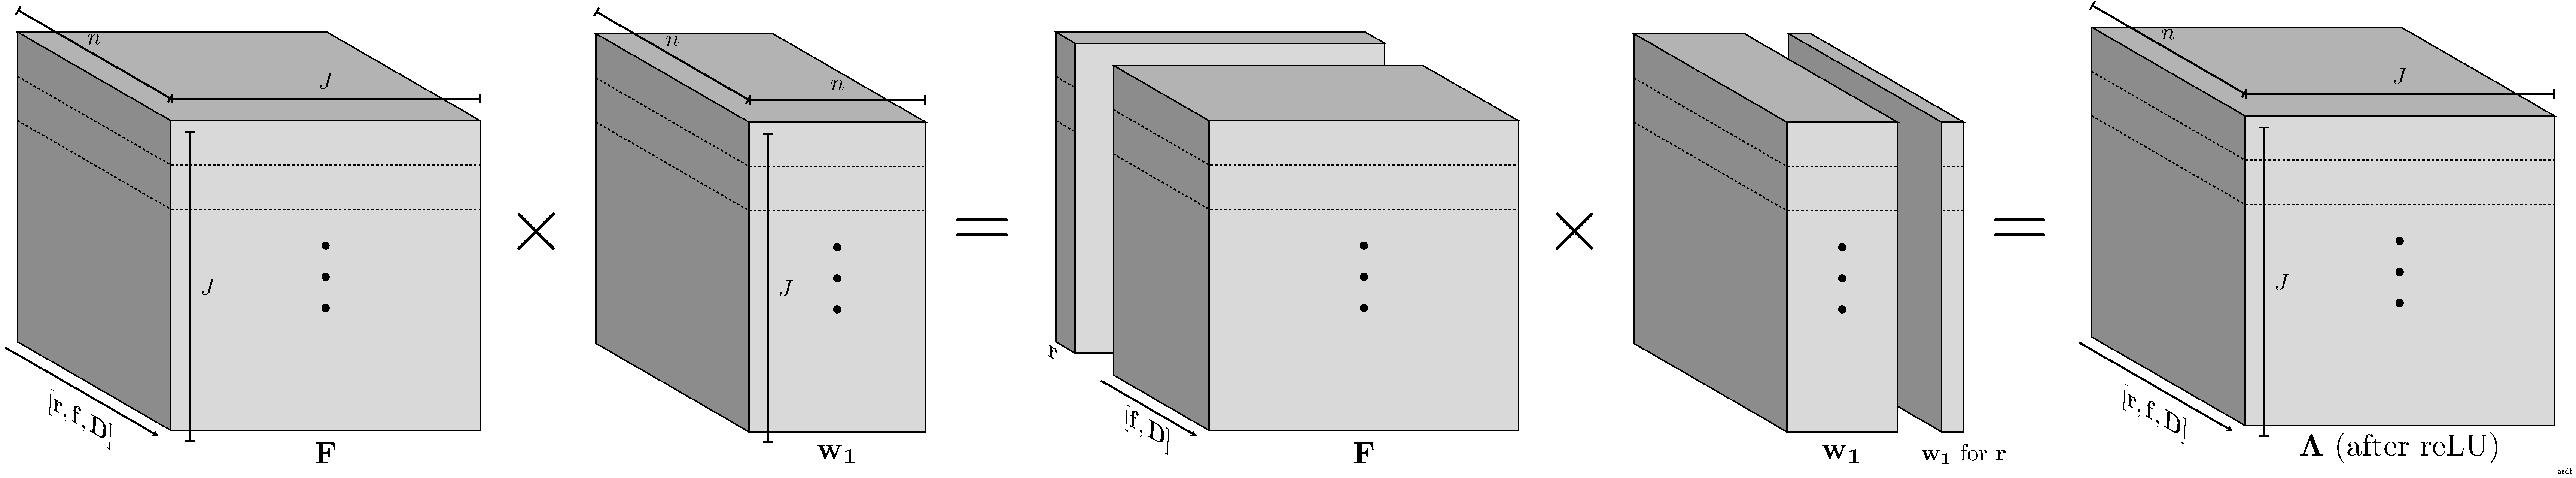
\includegraphics[width=\linewidth]{split_and_batch_multiply}
        \caption{Splitting and Batch Multiplying $\matr{F}$ and $\matr{w_1}$}
        \label{fig:Splitting and Batch Multiplying F and w1}
    \end{figure}    
    Although this preprocessing might seem applicable for the model in Identification Problem too, it does not apply fully. Since the weights $\matr{w_1}$ are updated on each iteration/epoch, we cannot multiply them with parts of $\matr{F}$ beforehand (Algorithm \ref{alg:Algorithm for the Identification Problem}). However, we can combine $\matr{D}$ and $\vect{f}$ in the preprocessing stage and simply append $\vect{r}[t]$ on each iteration, saving computation time.
    
    \subsubsection{Modeling the Linear Programming Problem in the Standard Format}
    The \texttt{scipy.optimize} module's \texttt{linprog} function requires that the arguments are in standard LP format. As discussed in \cref{sec:Calculating Rewards}, Equation \ref{eqn:lp_code_constrain_rewards} resembles the standard format more closely than \ref{eqn:lp_math_constrain_rewards}, but it may not be clear how so.\\
    
    Considering $\vect{u}$ and $\vect{r'}$ as variables $\vect{x}$, Equation \ref{eqn:lp_code_constrain_rewards} translates into Equation \ref{eqn:lp_matrix_rewards} ($J$ is the number of locations).
    \begin{equation} \label{eqn:lp_matrix_rewards}
    \begin{aligned}
    & \text{minimize}
    & & \begin{bmatrix}
    \vect{0_J}\\
    \vect{1_J}\\
    \end{bmatrix}^T
    \begin{bmatrix}
    \vect{r'}\\
    \vect{u}
    \end{bmatrix}\\ \\
    & \text{subject to}
    & & \begin{bmatrix}
    I_J & -I_J\\
    -I_J & -I_J\\
    \vect{1}^T_J & \vect{0}^T_J\\
    \end{bmatrix}
    \begin{bmatrix}
    \vect{r'}\\
    \vect{u}\\
    \end{bmatrix} \leq
    \begin{bmatrix}
    \vect{r}\\
    -\vect{r}\\
    \mathcal{R}\\
    \end{bmatrix}\\
    &&& r'_i, u_i \geq 0
    \end{aligned}
    \end{equation}
    
    \section{Strange GPU Speedup in LP Computation} \label{app:Strange GPU Speedup in LP Computation}
    Even though we intentionally transferred the rewards vector to and constrained it using \texttt{scipy.optimize} module's \texttt{linprog} function on the CPU, we obtained an unexpected GPU Speedup in the LP runtimes (see \cref{sec:PriProbRes - GPU} and Figure \ref{fig:Finding Rewards - Time taken by the LP}). Confounded by this weird behavior, we wanted to pinpoint the reason(s) because SciPy's function could not have differentiated between the configurations and delivered different results. However, since this was not our research's prime motive, we did not take a strong quantitative approach in determining the cause(s).
    
    \subsection{Possible Reasons for GPU Speedup} \label{app:Possible Reasons for GPU Speedup}
    There could have been many reasons for this bizarre behavior, including but not limited to:
    \begin{enumerate}
        \item SciPy's Optimize Module differentiating between configurations. This can be ruled out because the module could not have known the configuration during which it was called. This is because the configuration settings were applicable only on user-programmed operations, and needed to be explicitly stated - as mandated by Pytorch \cite{PTDocs}. SciPy's Optimize Module identifying the configurations is just supernatural.
        \item CPU ``set'' using exploiting more main memory than GPU ``set''. We suspected that since CPU ``set'' configuration's operations were executed solely on the CPU, the residing datasets could have used more main memory than when GPU ``set'' was running. This could have hampered the performance of LP with CPU ``set'', as the LP had lesser space to operate in. Unlike the 1\textsuperscript{st} possibility, this would have meant that CPU ``set'' was slowing down the LP, and not that GPU ``set'' was speeding up the LP.
        \item Neural network in CPU ``set'' using more CPU threads than that in GPU ``set''. The Intel i7-7700K processor is quad-core with 8 threads. Since Pytorch uses OpenMP \cite{PTDocs}, a parallel processing API for CPUs, we fancied the neural network to utilize more threads than that in GPU ``set'', thus allowing less available threads for the LP to run. 
        
        However, given that our scripts in Python did not explicitly use parallel programming with CPU ``set'' and the code was sequential, one could very well suggest that upon completion of the neural network, all threads should have been synchronized, after which the LP would have started. This would have meant that the LP's resources would have been independent of the neural network's resources, raising questions on this possibility.
    \end{enumerate}

    \subsection{LP Slowing Down or Speeding Up?} \label{app:LP Slowing Down or Speeding Up?}
    First we determined whether the LP runtime was being sped up with GPU ``set'' or slowed down with CPU ``set''. To test this, we created a copy of our Pricing Problem's model, which focused only on logging LP runtimes at each epoch. For a baseline comparison, we scripted the same LP \textit{without} the neural network, which gave us the \underline{original} runtimes for the LP (ran for equal number of epochs), without any involvement of Pytorch modules or functions. 
    
    Comparing the former runtimes (CPU and GPU ``set'') with `Only LP' runtime (independent script) in Figure \ref{fig:LP Runtime Example for Different Configurations}, we observed that the LP in the CPU ``set'' configuration took longer to execute than that in  `Only LP' setting during each epoch. We also noticed little to no interaction between the neural network in GPU ``set'' with the LP, as the runtimes of LP in GPU ``set'' were similar to those of LP in `Only LP' setting. This confirmed that CPU ``set'' was slowing down the LP and GPU ``set'' was not speeding it up. But why?
    \begin{figure}[!htbp]
        \centering
        \begin{tikzpicture}
        \begin{axis}[
            width=\textwidth,
            height=8cm,
            xlabel=Epochs,
            ylabel=Time/s,
            scaled y ticks = false,
            grid=both,
            every axis plot/.append style={very thick},
        ]
        \addplot[red] table [col sep=comma,x=epoch, y=cpuset]{datafiles/lp_time_logs.csv};
        \addlegendentry{CPU ``set''}
        
        \addplot[blue] table [col sep=comma,x=epoch, y=gpuset]{datafiles/lp_time_logs.csv};
        \addlegendentry{GPU ``set''}
        
        \addplot[brown] table [col sep=comma,x=epoch, y=onlylp]{datafiles/lp_time_logs.csv};
        \addlegendentry{`Only LP'}
        
        \end{axis}
        \end{tikzpicture}
        \caption[LP Runtime Example for Different Configurations]{LP Runtime Example for Different Configurations: LPs in both CPU and GPU ``set'' start running slowly, but pick up speed after $\approx$ 20 epochs. We could not explain the presence of spikes in LP runtimes of CPU ``set'' and their absence in GPU ``set''. The test was done on a random dataset for 200 epochs, while the other experiment specifications were same as in \cref{sec:Experiment Specifications}.}
        \label{fig:LP Runtime Example for Different Configurations}
    \end{figure}
    
    \subsection{CPU and Main Memory Usage} \label{app:CPU and Main Memory Usage}
    While logging the LP runtimes in \cref{sec:LP Slowing Down or Speeding Up?}, we also recorded an estimate of the amount of computer resources both configurations were using. Using the \texttt{top} package in Ubuntu, we polled the resource monitor every 0.1 seconds while the python script was running\footnote{\label{foo:logs not epochs} Running processes were polled every 0.1 seconds - contributing to a `log'. The longer the script ran, the more logs collected.}. Figures \ref{fig:CPU Usage by Different Configurations} and \ref{fig:Main Memory Usage by Different Configurations} shows how much main memory and CPU resource each setting was using.
    
    It is fascinating to see that CPU ``set'' constantly used more than 4 out of 8 available threads, i.e., $>400\%$ CPU usage, during execution, while GPU ``set'' only used a single thread. Also, since we polled at every 0.1 second, and the LP took a minimum of 0.14 seconds (Figure \ref{fig:LP Runtime Example for Different Configurations}), the data displayed in Figure \ref{fig:CPU Usage by Different Configurations} must show resource use \textit{while} the LP was running. Considering that the LP in `Only LP' setting only used a single thread (100\%), it makes sense that GPU ``set'' would use 1 thread for execution - the neural network operations were performed on the GPU, leaving the CPU empty for management and LP. On the other hand, it is apparent that CPU ``set'' had multi-threaded operations running simultaneously, even though we reasoned its low possibility (\#3 in \cref{sec:Possible Reasons for GPU Speedup}). Since we know from the `Only LP' setting that the LP only used a single thread, the other threads in CPU ``set'' must have been the neural network. Although this counters our reasoning that the neural network threads should have synchronized before the LP started, it seems that those threads were still active. While we cannot explain this behavior, this activity does not impact correctness, as found from optimization tests on CPU ``set''\footnote{CPU ``set'' tests were done for optimization on original datasets to check this. Since we got the same results as for GPU ``set'' optimization tests \cref{sec:PriProbRes - Optimization}, the results are not shown in the report.} (same optimization figures as obtained for GPU ``set'' - \cref{sec:PriProbRes - Optimization}).
    
    On the other hand, GPU ``set'' was using 10 times as much main memory as CPU ``set'' or `Only LP', even though all matrix operations were executed and stored on the GPU. Not only this is weird, but it is also opposite of what we expected to happen - CPU ``set'' using more main memory and hampering LP performance. It is ironic that the LP performs better (even as good as `Only LP') on GPU ``set'' even when the configuration uses a lot more main memory than CPU ``set''. Clearly, the main memory usage cannot be a criterion for assessing LP performance on different configurations.
    \begin{figure}[!htbp]
        \centering
        \begin{minipage}{.49\textwidth}
            \centering
            \begin{tikzpicture}
            \begin{axis}[
            name=cpuusage-cpuset,
            width=\textwidth,
            enlarge x limits=0.15,
            no markers,
            ymax=800,
            ymin=0,
            ]
            \addplot+[fill=red, opacity=.4] table [col sep=comma,x=epoch, y=cpu]{datafiles/ext_cpu_cpuset.csv} \closedcycle;
            
            \addplot+[very thick, red!50!black] table [col sep=comma,x=epoch, y=cpu]{datafiles/ext_cpu_cpuset.csv};
            
            \end{axis}
            
            \begin{axis}[
            name=cpuusage-gpuset,
            at=(cpuusage-cpuset.below south west), anchor=above north west,
            width=\textwidth,
            enlarge x limits=0.15,
            no markers,
            ylabel={CPU Usage/\%},
            ymax=200,
            ymin=0,
            ]
            \addplot+[fill=blue, opacity=.4] table [col sep=comma,x=epoch, y=cpu]{datafiles/ext_cpu_gpuset.csv} \closedcycle;
            
            \addplot+[very thick, blue!50!black] table [col sep=comma,x=epoch, y=cpu]{datafiles/ext_cpu_gpuset.csv};
            \end{axis}
            
            \begin{axis}[
            name=cpuusage-onlylp,
            at=(cpuusage-gpuset.below south west), anchor=above north west,
            width=\textwidth,
            enlarge x limits=0.15,
            no markers,
            xlabel={Logs},
            ymax=200,
            ymin=0,
            ]
            \addplot+[fill=green, opacity=.4] table [col sep=comma,x=epoch, y=cpu]{datafiles/ext_onlylp.csv} \closedcycle;
            
            \addplot+[very thick, green!50!black] table [col sep=comma,x=epoch, y=cpu]{datafiles/ext_onlylp.csv};
            \end{axis}
            \end{tikzpicture}
            \caption[CPU Usage by Different Configurations]{CPU Usage by Different Configurations\textsuperscript{\ref{foo:logs not epochs}}: From top - CPU ``set'', GPU ``set'', `Only LP'. CPU Usage for GPU ``set'' and `Only LP' are very similar as operations other than the LP run on the GPU.}
            \label{fig:CPU Usage by Different Configurations}
        \end{minipage}\hfill
        \begin{minipage}{.49\textwidth}
            \centering
            \begin{tikzpicture}
            \begin{axis}[
            name=memusage-cpuset,
            width=\textwidth,
            enlarge x limits=0.15,
            no markers,
            ymax=1,
            ymin=0,
            ]
            \addplot+[fill=red, opacity=.4] table [col sep=comma,x=epoch, y=mem]{datafiles/ext_cpu_cpuset.csv} \closedcycle;
            
            \addplot+[very thick, red!50!black] table [col sep=comma,x=epoch, y=mem]{datafiles/ext_cpu_cpuset.csv};
            
            \end{axis}
            
            \begin{axis}[
            name=memusage-gpuset,
            at=(memusage-cpuset.below south west), anchor=above north west,
            width=\textwidth,
            enlarge x limits=0.15,
            no markers,
            ylabel={Main Memory Usage/\%},
            ymax=10,
            ymin=0,
            ]
            \addplot+[fill=blue, opacity=.4] table [col sep=comma,x=epoch, y=mem]{datafiles/ext_cpu_gpuset.csv} \closedcycle;
            
            \addplot+[very thick, blue!50!black] table [col sep=comma,x=epoch, y=mem]{datafiles/ext_cpu_gpuset.csv};
            \end{axis}
            
            \begin{axis}[
            name=memusage-onlylp,
            at=(memusage-gpuset.below south west), anchor=above north west,
            width=\textwidth,
            enlarge x limits=0.15,
            no markers,
            xlabel={Logs},
            ymax=1,
            ymin=0,
            ]
            \addplot+[fill=green, opacity=.4] table [col sep=comma,x=epoch, y=mem]{datafiles/ext_onlylp.csv} \closedcycle;
            
            \addplot+[very thick, green!50!black] table [col sep=comma,x=epoch, y=mem]{datafiles/ext_onlylp.csv};
            \end{axis}
            \end{tikzpicture}
            \caption[Main Memory Usage by Different Configurations]{Main Memory Usage by Different Configurations\textsuperscript{\ref{foo:logs not epochs}}: From top - CPU ``set'', GPU ``set'', `Only LP'. The neural network doesn't occupy much main memory in CPU ``set'' - could be due to Python/Pytorch's garbage collection.}
            \label{fig:Main Memory Usage by Different Configurations}
        \end{minipage}
    \end{figure}

    \subsubsection{Inexplicable Behavior} \label{app:Inexplicable Behavior}
    The machine's resource logs while model execution defy our expectations starkly. Elaborated in \cref{sec:CPU and Main Memory Usage}, it is clear that Main Memory Usage does not explain the strange GPU Speedup in LP runtimes for CPU and GPU ``set''; instead, main memory logs show the opposite picture - with GPU ``set'' using $\approx$ 10 times as much main memory as CPU ``set'' or `Only LP'.
    
    On the other hand, CPU Usage logs do correspond with our LP runtime observations, but the former phenomenon is inexplicable, at least from our side. We believe that the neural network should stop executing and the threads should synchronize, before the LP starts. The LP on CPU ``set'' should then use just 1 thread, as with `Only LP' setting, forming high spikes in the CPU usage graph (top, Figure \ref{fig:CPU Usage by Different Configurations}). At odds with what we expect, the CPU Usage graph shows constant use of 4-5 threads with tiny spikes, which are natural, indicating that the neural network's threads were running \textit{along with} the LP. While this would have targeted the model's correctness on CPU ``set'' config., the results we obtained are same as those with GPU ``set''.
    
    Therefore, while CPU usage logs for the configurations might explain the strange GPU Speedup, CPU usage for CPU ``set'' is itself strange and inexplicable. Additionally, main memory usage in GPU ``set'' is inexplicably high. Although both these behaviors could be caused by Pytorch's implementation specifics, we cannot ensure this possibility. Further research and suggestions are welcome.
\end{appendices}
\end{document}